\chapter{SISTAL}

% \subsection{Situación Actual}

% \subsection{Análisis FODA}

% \subsection{Solución Propuesta}

\section{Diseño del Sistema Actual}

\subsection{Diagrama de Casos de Uso}

\subsection{Diagrama de Bases de Datos}

\begin{figure}[htbp]
    \centering
    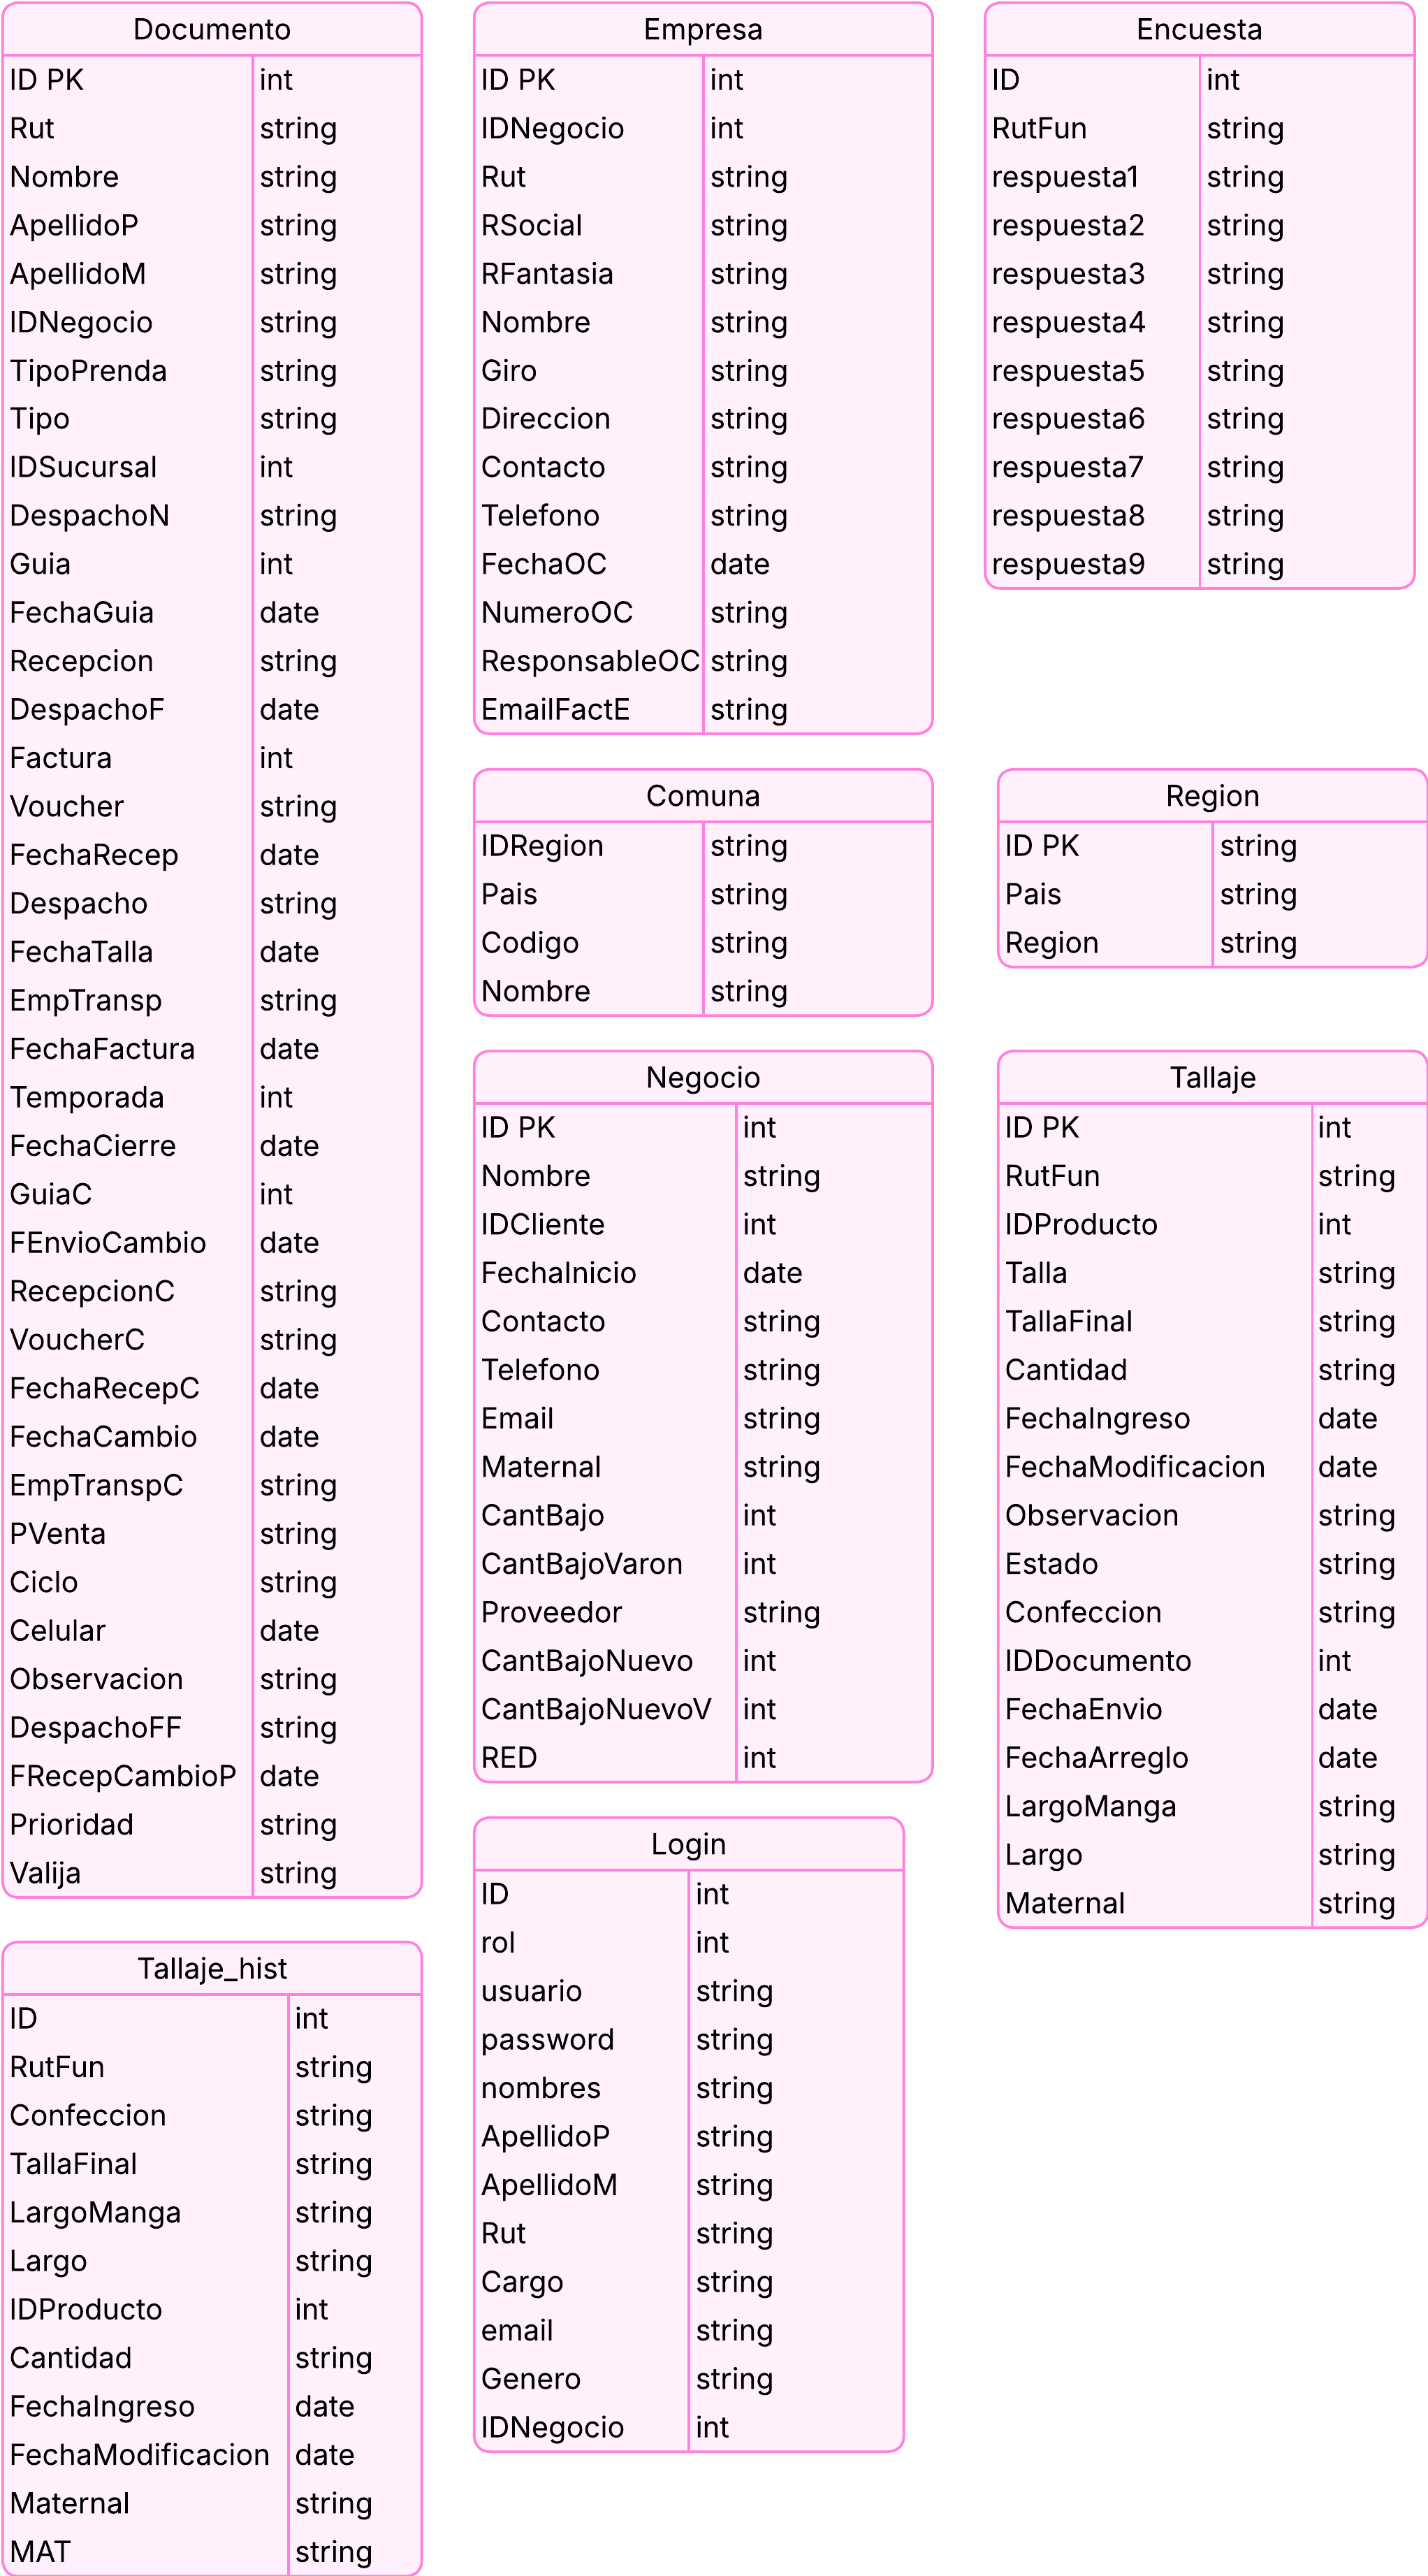
\includegraphics[height=0.7\textheight]{figuras/diagramas-actuales/diagrama-bdd-1}
    \caption{Diagrama físico de bases de datos del sistema actual (Parte 1)}
    \label{fig:diagrama-bdd-1-actual}
\end{figure}

\begin{figure}[htbp]
    \centering
    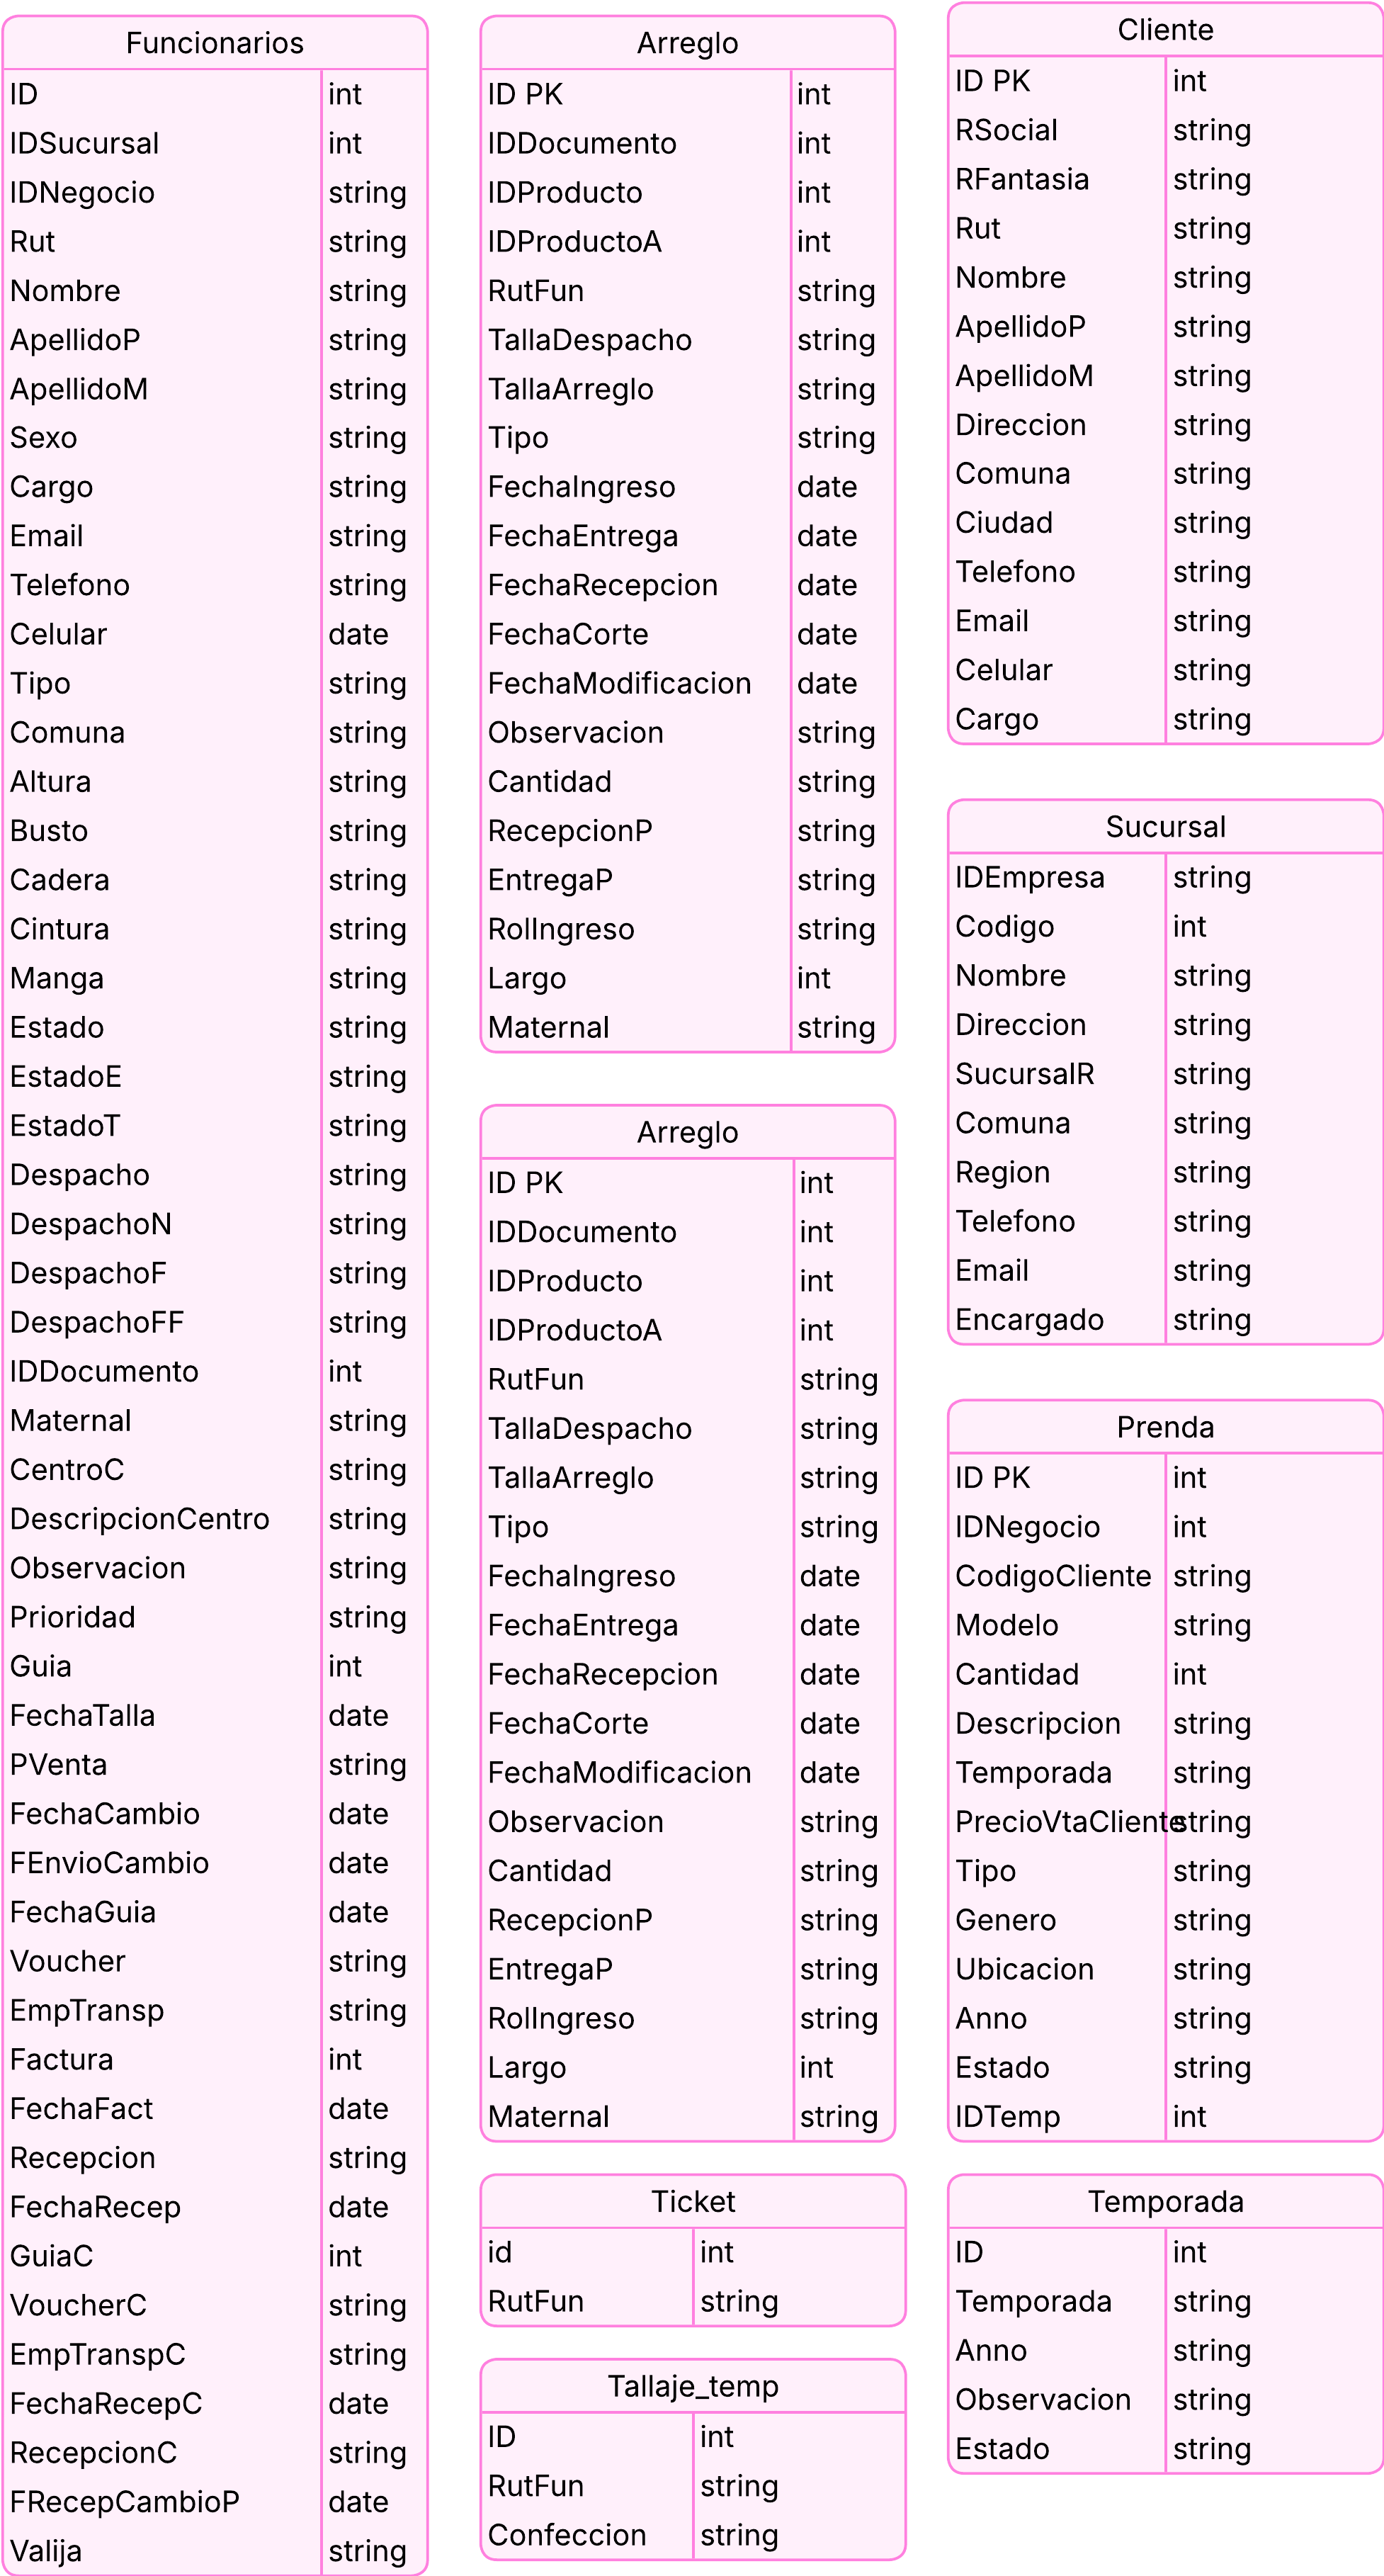
\includegraphics[height=0.7\textheight]{figuras/diagramas-actuales/diagrama-bdd-2}
    \caption{Diagrama físico de bases de datos del sistema actual (Parte 2)}
    \label{fig:diagrama-bdd-2-actual}
\end{figure}


\subsection{Diagrama de Flujo}

\subsection{Diagrama de Arquitectura}

\begin{figure}[htbp]
    \centering
    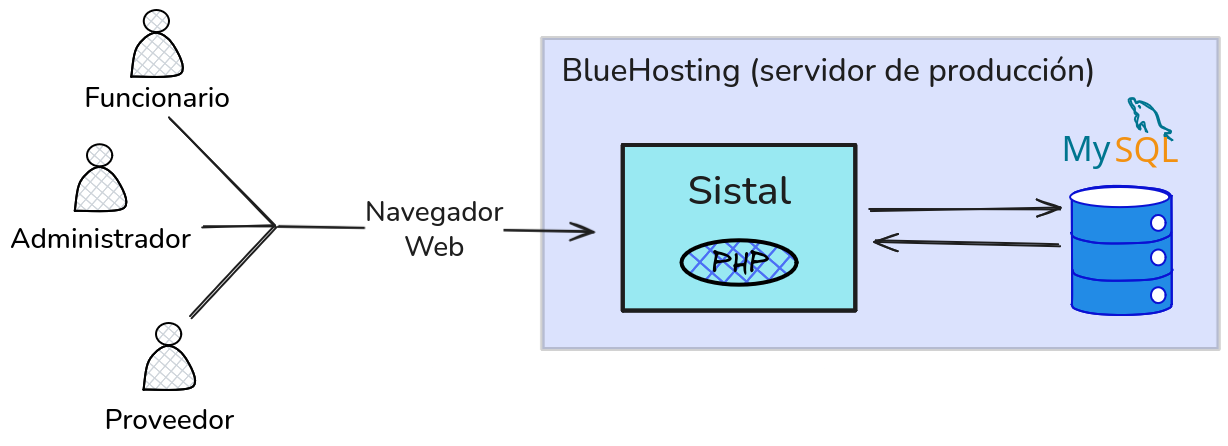
\includegraphics[width=0.9\textwidth]{figuras/diagramas-actuales/diagrama-de-arquitectura}
    \caption{Diagrama de arquitectura del sistema actual}
    \label{fig:diagrama-arq-actual}
\end{figure}

\subsection{Diagrama de Despliegue}

\begin{figure}[htbp]
    \centering
    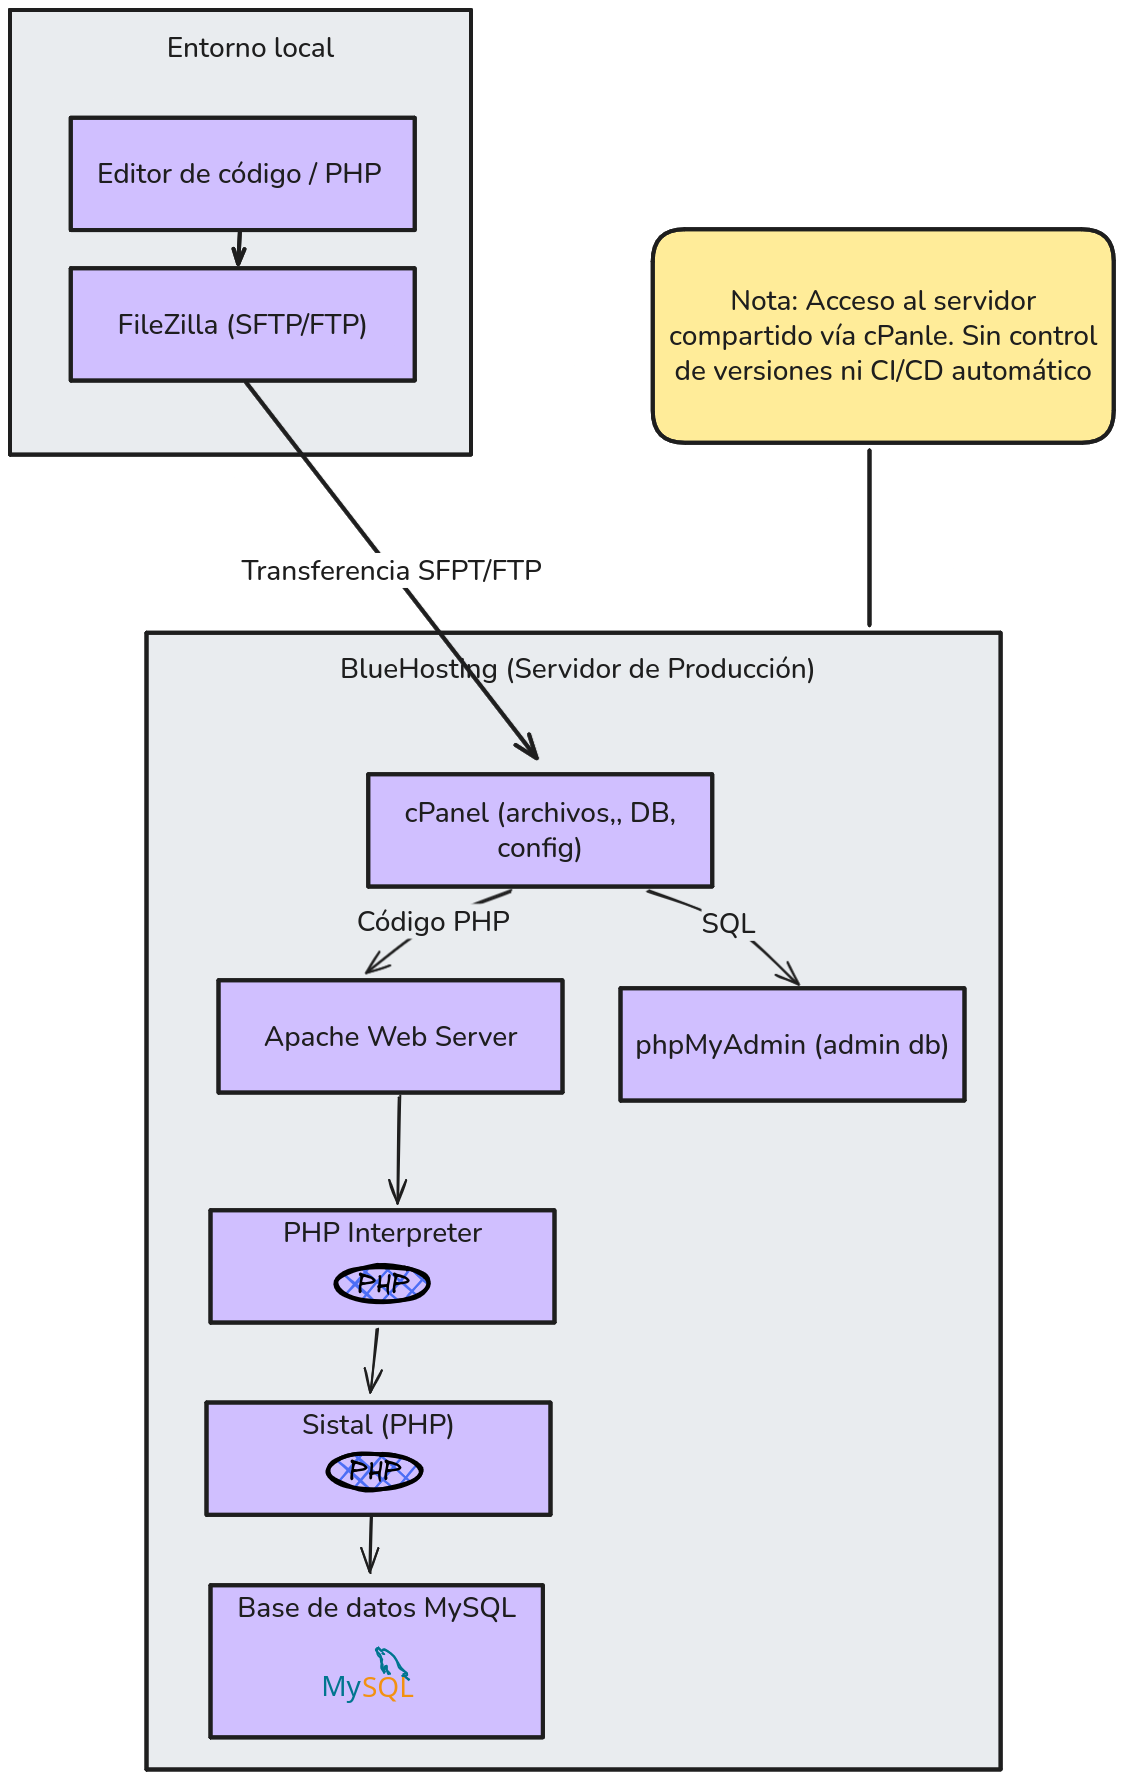
\includegraphics[width=0.5\textwidth]{figuras/diagramas-actuales/diagrama-de-despliegue}
    \caption{Diagrama de despliegue del sistema actual}
    \label{fig:diagrama-despliegue-actual}
\end{figure}

